Lets start from dense (hexagonal) packing of disks on plane.
\begin{center}
	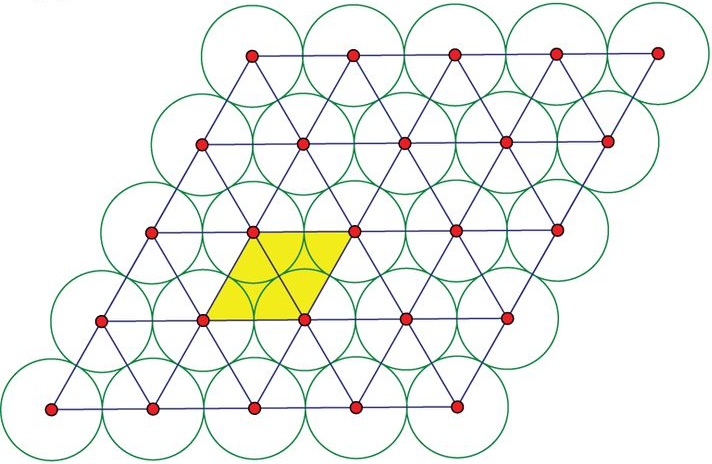
\includegraphics[width=0.5\linewidth]{./lect26/1.png}
\end{center}
Area of each disk is 
$$A(D) = \pi R^2$$
and area of ``triangle'' is
$$A(T) = \left(\sqrt{3} - \frac{\pi}{2}\right)R^2$$
Total covered area is
$$\frac{A(D)}{A(D) + 2A(T)} = \frac{\pi}{\sqrt{3} - \frac{\pi}{2}} \approx 0.907$$
Thus choosing random packing (two coordinates of center of one disk), probability of point to be not covered is
$$P(x_i) \approx 0.093$$
Then probability that at least one point is uncovered
$$P\left(\left\{ x_n\right\}  \right) \leq 10 \cdot P(x_i) = 10 \cdot 0.093 = 0.93 < 1$$
i.e. exist packing for which all 10 are covered.

\subsection{Secretary problem}
 In this game Alice, the informed player, writes secretly distinct numbers on $n$ cards. Bob, the stopping player, observes the actual values and can stop turning cards whenever he wants, winning if the last card turned has the overall maximal number.
 
 
Call strategy $j$ (for $j>0$) - to skip first $j$ numbers and then choose the first number bigger then all previous numbers. Denote by $W$ event of winning. What is $P_j(W)$ - probability to win using strategy $j$.
Denote by $A_k$ event that $k^{th}$ number is biggest.
$$P_j(A_k) = \frac{1}{n}$$
Find probability of winning via full probability
$$P_j(W) = \sum_{k=1}^n P(A_k)P(W|A_k) = \frac{1}{n} \sum_{k=1}^n P_j(W|A_k)$$
Now, if $1\leq k \leq j$,
$$P_j(W|A_k) = 0 $$
In other case, if maximum of first $k-1$ numbers is in first $j$ numbers, we win, else we lose, i.e.
$$P_j(W|A_k)  = \frac{j}{k-1}$$
Back to probability
$$P_j(W) =  \frac{1}{n} \sum_{k=j+1}^n \frac{j}{k-1}$$
Now lets perform asymptotic analysis for $j = \left[xn\right]$, $0<x<1$:

$$ \sum_{k=[xn]+1}^n \frac{1}{k-1} = \sum_{k=2}^n \frac{1}{k-1} - \sum_{k=2}^{[xn]} \frac{1}{k-1} \approx \log n - \log xn = -\log x$$
Thus
$$P_j(W) \approx -\frac{[xn]}{n} \log x = -x \log x$$
To maximize probability:
$$P'_j(W) = \log x + 1$$
$$\log x = -1$$
$$x = \frac{1}{e} \approx 0.368$$
And probability to win is 
$$P_j(W)  = -e^{-1} \log e^{-1} = e^{-1}\approx 0.368$$